Approximation algorithms can obtain significant benefits from using customized
scheduling policies since they follow important statistical properties and thus
can trade correctness for faster convergence. An example of such algorithm is
the Loopy Belief Propagation (LBP)~\cite{Murphy99loopybelief}. LBP is an
approximate inference algorithm used in graphical models with cycles which
employs a sum-product message passing algorithm where nodes exchange messages
with their immediate neighbors and apply some computations to the messages
received.

\begin{figure}[h]
   \begin{center}
      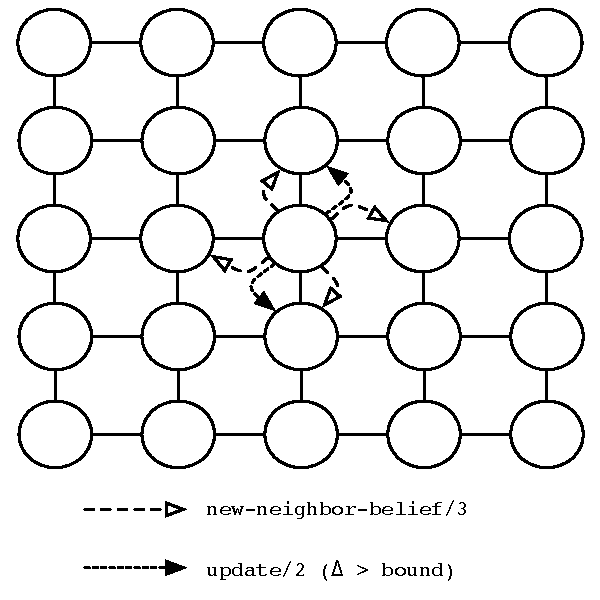
\includegraphics[width=0.3\textwidth]{figures/bp/bp.pdf}
   \end{center}

   \mycap{LBP communication patterns. \code{new-neighbor-belief} facts are
   sent to the neighborhood when the node's belief value is updated. If the new
   value sent to the neighbor differs significantly from the value sent before
   the current the round, then an \code{update} fact is also sent (to the node
   above and below in this case).}

\label{fig:coordination:bp}
\end{figure}

LBP is an algorithm that maps very well to the graph-based model of LM. The
original algorithm computes the belief of all nodes using several iterations
with synchronization between iterations. However, it is possible to avoid the
synchronization step, if we take advantage of the fact that LBP will converge
even when using an asynchronous approach. So, instead of computing the belief
iteratively, we keep track of all messages sent/received (and overwrite them
when we receive a new one) and recompute the belief asynchronously.
Figure~\ref{fig:coordination:bp} presents the communication patterns of the
program, while Fig.~\ref{code:coordination:bp} presents the LM code for the
asynchronous version of LBP.

\begin{figure}[ht]
\begin{Verbatim}[numbers=left, fontsize=\codesize, commandchars=\*\#\&]
type list float belief.*hfill// Type declaration.

type potential(node, belief).*hfill// Predicate declaration
type edge(node, node).
type linear neighbor-belief(node, node, belief).
type linear new-neighbor-belief(node, node, belief).
type linear sent-neighbor-belief(node, node, belief).
type linear check-residual(node, float, node).
type linear belief(node, belief).
type linear update-messages(node, belief).
type linear update(node).

neighbor-belief(A, B, Belief),*label#line:coord:bp_first1&*hfill// Rule 1: update neighbor belief value
new-neighbor-belief(A, B, NewBelief)
   -o neighbor-belief(A, B, NewBelief).*label#line:coord:bp_first2&

check-residual(A, Residual, B),*label#line:coord:bp_check1&*hfill// Rule 2: check residual
Residual > bound
   -o update(B).

check-residual(A, _, _) -o 1.*label#line:coord:bp_check2&*hfill// Rule 3: check residual

update-messages(A, NewBelief),*hfill// Rule 4: compute belief to be sent to a neighbor node*label#line:coord:bp_iterate1&
   -o {B, OldIn, OldOut, Cavity, Convolved, OutMessage, Residual |
         !edge(A, B),
         neighbor-belief(A, B, OldIn),
         sent-neighbor-belief(A, B, OldOut),
         Cavity = normalize(divide(NewBelief, OldIn)),
         Convolved = normalize(convolve(global-potential, Cavity)),
         OutMessage = damp(Convolved, OldOut, damping)
         Residual = residual(OutMessage, OldOut)
         -o check-residual(A, Residual, B),
            new-neighbor-belief(B, A, OutMessage),
            neighbor-belief(A, B, OldIn),
            sent-neighbor-belief(A, B, OutMessage)}.*label#line:coord:bp_iterate2&

*label#line:coord:bp_last1&
update(A), update(A) -o update(A).*label#line:coord:bp_update&*hfill// Rule 5: prune redundant update operations

update(A),*hfill// Rule 6: initiate update operation*label#line:coord:bp_update1&
!potential(A, Potential),
belief(A, MyBelief)
   -o [sum Potential => Belief; B, Belief |*label#line:coord:bp_agg1&
         neighbor-belief(A, B, Belief) -o
         neighbor-belief(A, B, Belief) ->
         Normalized = normalizestruct(Belief),
         update-messages(A, Normalized), belief(A, Normalized)].*label#line:coord:bp_last2&*label#line:coord:bp_update2&*label#line:coord:bp_agg2&
\end{Verbatim}

\mycap{LM code for the asynchronous version of the Loopy Belief Propagation
problem.}

\label{code:coordination:bp}
\end{figure}

\clearpage

Belief values are arrays of floats and are represented by \code{belief/2} facts.
The first rule (lines~\ref{line:coord:bp_first1}-\ref{line:coord:bp_first2})
updates a given neighbor belief whenever a new belief value is received. This is
the highest priority rule since we want to update the neighbor beliefs before
doing anything else. In order to store the belief values of the neighbor nodes,
we use \code{neighbor-belief/3} facts, where the second argument is the neighbor
address and the third argument is the belief value.

The last two rules (lines~\ref{line:coord:bp_last1}-\ref{line:coord:bp_last2})
update the belief value of a node. An \code{update} fact starts the process.
The first rule (line~\ref{line:coord:bp_update}) simply removes redundant
\code{update} facts and the second rule
(lines~\ref{line:coord:bp_update1}-\ref{line:coord:bp_update2}) performs the
belief update by aggregating all the neighbor belief values. The aggregate in
lines~\ref{line:coord:bp_agg1}-\ref{line:coord:bp_agg2} also derives copies of
the neighbors beliefs that need to be consumed in order to compute the belief
value that is going to be sent to the target neighbor. The aggregate uses a
custom accumulator that takes two arrays and adds the floating point numbers at
each index of the array.

The rule in lines~\ref{line:coord:bp_iterate1}-\ref{line:coord:bp_iterate2}
iterates through the neighbor belief values and sends new belief values by
performing the appropriate computations on the new belief value of the current
node and on the belief value sent previously. For each neighbor update, we also
check in lines~\ref{line:coord:bp_check1}-\ref{line:coord:bp_check2} if the
change in belief values is greater than \code{bound} (a program constant) and
then force the neighbor nodes to update their belief values by deriving
\code{update(B)}. This allows neighbor nodes to use updated neighbor values and
recompute their own belief values using more up-to-date information. The
computation of belief values will then start to converge to their true belief
values, independently of the node scheduling used.

However, if we prioritize nodes that receive new neighbor belief values with a
larger \code{Residual} then we may converge faster.
Figure~\ref{code:coordination:improved_bp} shows the fourth rule modified with a
\code{add-priority} fact, which increases the priority of neighbor nodes when
the source node has large changes in its belief value.

\begin{figure}[h!]
\begin{Verbatim}[numbers=left,commandchars=\\\{\},fontsize=\codesize]
update-messages(A, NewBelief),*hfill// Rule 4: compute belief to be sent to a neighbor node
   -o \{B, OldIn, OldOut, Cavity, Convolved, OutMessage, Residual |
         !edge(A, B),
         neighbor-belief(A, B, OldIn),
         sent-neighbor-belief(A, B, OldOut),
         Cavity = normalize(divide(NewBelief, OldIn)),
         Convolved = normalize(convolve(global-potential, Cavity)),
         OutMessage = damp(Convolved, OldOut, damping)
         Residual = residual(OutMessage, OldOut)
         -o check-residual(A, Residual, B),
            new-neighbor-belief(B, A, OutMessage),
            neighbor-belief(A, B, OldIn),
            \underline{add-priority(B, Residual)},
            sent-neighbor-belief(A, B, OutMessage)\}.
\end{Verbatim}
\mycap{Extending the LBP program with priorities.}
\label{code:coordination:improved_bp}
\end{figure}


The proposed asynchronous approach has shown to be an improvement over the
synchronous version because it leads to faster convergence time. An improved
evaluation strategy is the Splash Belief
Propagation~(SBP)~\cite{Gonzalez+al:aistats09paraml}, where belief values are
computed asynchronously by first building a tree and then by updating the
beliefs of each node twice, first from the leaves to the root and then from the
root to the leaves. These \emph{splash trees} are built by starting at a node
whose belief changed the most in the last update. The trees must be built
iteratively until convergence is achieved.

In an environment with $T$ threads, it is then possible to build $T$ splash
trees concurrently. First, we partition the nodes into $T$ regions and then
assign each region to a thread. A thread is then responsible for iteratively
building splash trees on that region until convergence is reached.
Fig.~\ref{fig:threads:splash_bp} shows a grid of nodes that has been partitioned
in two regions where splash trees will be built. To build a splash tree, a
thread starts from the highest priority node (the tree's root) from its region
and then performs a breadth-first search from that node to construct the rest of
the tree. The belief values are then computed in order.

\begin{figure}[ht]
   \begin{center}
      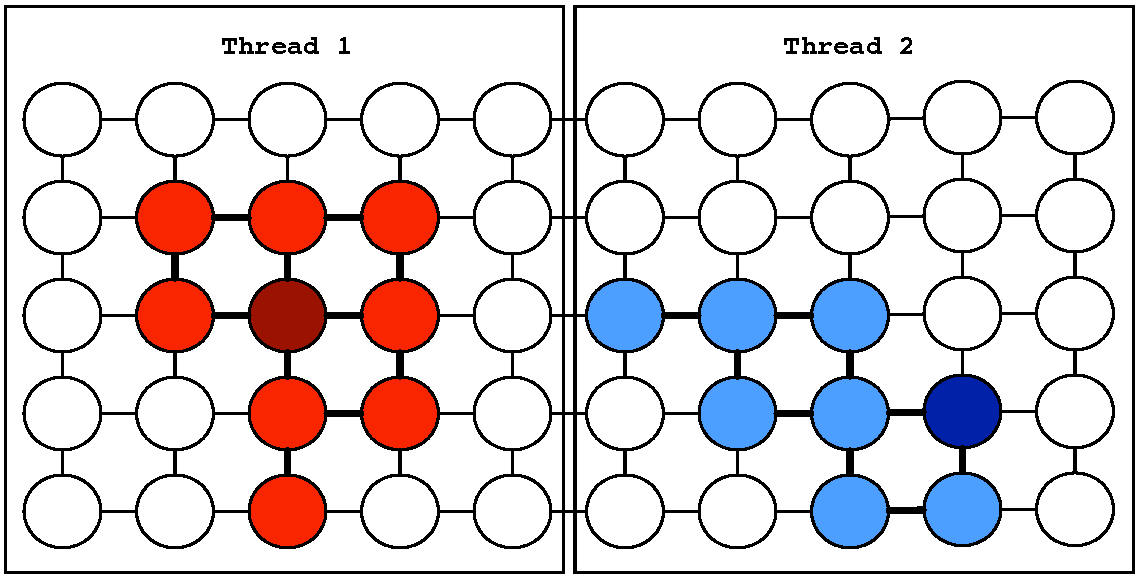
\includegraphics[width=0.7\linewidth]{figures/threads/splash_bp}
   \end{center}
   \mycap{Creating splash trees using two threads. The graph is
      partitioned into two regions and each thread is able to build separate
   splash trees starting from the highest priority node.}
   \label{fig:threads:splash_bp}
\end{figure}

The LM implementation for SBP is shown in Fig.~\ref{code:threads:sbp}. First,
in lines \ref{line:threads:splash_part1}-\ref{line:threads:splash_part2}, we
partition the nodes into regions using \code{set-thread} and then we start the
creation of the first splash tree (line~\ref{line:threads:splash_first}) by
deriving \code{start-tree(T)}.  The remaining phases of the algorithm are
explained next.

\begin{figure}[!htb]
\begin{Verbatim}[numbers=left,commandchars=*\{\},fontsize=\codesize]
type list node tree.

type linear partitioning(thread, int).*hfill// Number of nodes to receive.
type linear start-tree(thread).
type linear new-tree(thread, tree, tree).
type linear expand-tree(thread, tree).
type linear first-phase(thread, tree, tree).
type linear second-phase(thread, tree).
type linear start(node).

start(A).
partitioning(T, @world / @threads).*hfill// Move @world/@threads nodes.

!coord(A, X, Y), start(A)*hfill// Moving this node.*label{line:threads:splash_part1}
   -o set-thread(A, grid(X, Y)).
just-moved(A), partitioning(T, Left)*hfill// Thread received another node.
   -o partitioning(T, Left - 1).
partitioning(T, 0) -o start-tree(T).*label{line:threads:splash_part2}*label{line:threads:splash_first}

start-tree(T),*label{line:threads:splash_building1} priority(A, P), P > 0.0 *hfill{} // Tree building
   -o priority(A, P), expand-tree(T, [A], []).*label{line:threads:splash_building2}
expand-tree(T, [A | All], Next)
   -o thread-id(A, Id),
      [collect => L ; | !edge(A, L), ~ L in All, ~ L in Next,*label{line:threads:splash_agg1} priority(L, P), P > 0.0,
         thread-id(L, Id2), Id1 = Id2 -o priority(L, P), thread-id(L, Id2) ->
         new-tree(T, [A | All],
            if len(All) + 1 >= maxnodes then [] else Next ++ L end)].*label{line:threads:splash_agg2}*label{line:threads:splash_next}

new-tree(T, [A | All], [])
   -o schedule-next(A), first-phase(T, reverse([A | All]), [A | All]).*label{line:threads:splash_first_phase}
new-tree(T, All, [B | Next])
   -o schedule-next(B), expand-tree(T, [B | All], Next).

first-phase(T, [A], [A]), running(T, A) *hfill{} // First phase
   -o running(T, A), update(A), remove-priority(A), start-tree(T).
first-phase(T, [A, B | Next], [A]), running(T, A)
   -o running(T, A), update(A), schedule-next(B), second-phase(T, [B | Next]).*label{line:threads:splash_first_update1}
first-phase(T, All, [A, B | Next]), running(T, A)
   -o running(T, A), update(A), schedule-next(B), first-phase(T, All, [B | Next]).*label{line:threads:splash_first_update2}

second-phase(T, [A]), running(T, A) *hfill{} // Second phase
   -o running(T, A), update(A), remove-priority(A), start-tree(T).*label{line:threads:splash_second_update1}
second-phase(T, [A, B | Next]), running(T, A)
   -o running(T, A), update(A), schedule-next(B), second-phase(T, [B | Next]).*label{line:threads:splash_second_update2}
\end{Verbatim}

   \mycap{LM code for the Splash Belief Propagation program.}
  \label{code:threads:sbp}
\end{figure}

\begin{description}

   \item[Tree building:] Starts after the rule in lines
      \ref{line:threads:splash_building1}-\ref{line:threads:splash_building2} is
      derived. Since the thread always picks the highest priority node, we start
      by adding that node to the list that represents the tree. In lines
      \ref{line:threads:splash_agg1}-\ref{line:threads:splash_agg2}, we use an
      aggregate to gather all the neighbor nodes that have a positive priority
      (due to a new belief update) and are in the same thread. Nodes are
      collected into list \code{L} and appended to list \code{Next}
      (line~\ref{line:threads:splash_next}).

   \item[First phase:] When the number of nodes in the tree reaches a certain
      limit, a \code{first-phase} is generated to update the beliefs of all
      nodes in the tree (line~\ref{line:threads:splash_first_phase}). As the
      nodes are updated, starting from the leaves and ending at the root, an
      \code{update} fact is derived to update the belief values
      (lines~\ref{line:threads:splash_first_update1}
      and~\ref{line:threads:splash_first_update2}).

   \item[Second phase:] Performs the computation of beliefs from the root to the
      leaves and the belief values are updated a second time
      (lines~\ref{line:threads:splash_second_update1}
      and~\ref{line:threads:splash_second_update2}).

\end{description}

SBP is also implemented in GraphLab~\cite{GraphLab2010}, a C++ framework for
writing machine learning algorithms. GraphLab provides different schedulers that
change how machine learning algorithms are computed and one of the available
schedulers is the \textbf{splash} scheduler, which implements the scheduling
described above. For comparison purposes with LM, we also experimented with two
other GraphLab schedulers: \textbf{fifo}, a first-in first-out scheduler and
\textbf{multiqueue}, a first-in first-out scheduler that also allows for
\textit{work stealing} (we used 1 queue per thread).

The default LM scheduling policy of LM is somewhat similar to both the
\textbf{fifo} and the \textbf{multiqueue} schedulers, however, since LM also
implements node stealing by default, the \textbf{multiqueue} scheduler will be
our main focus. We measured the run time of LBP and SBP for both LM and
GraphLab. For SBP, we used splash trees of 100 nodes in both systems.

Fig.~\ref{fig:threads:results_splash} compares the performance of the LBP
program in LM against both the \textbf{fifo} and \textbf{multiqueue} schedulers.
The results show that GraphLab's \textbf{fifo} scheduler performance
deteriorates with more 10 threads, while both LM and \textbf{multiqueue} tend to
scale well and have a similar behavior. For 1 thread, LM is about 1.5 times
slower than GraphLab but that ratio increases to about to about 2 once the
number of threads increases. We think this is because the LBP program is fairly
sensitive to scheduling policies and the \textbf{multiqueue} scheduler is better
than LM's default scheduling policy.

\begin{figure}[]
        \centering
        \begin{subfigure}[b]{\plotsize\textwidth}
           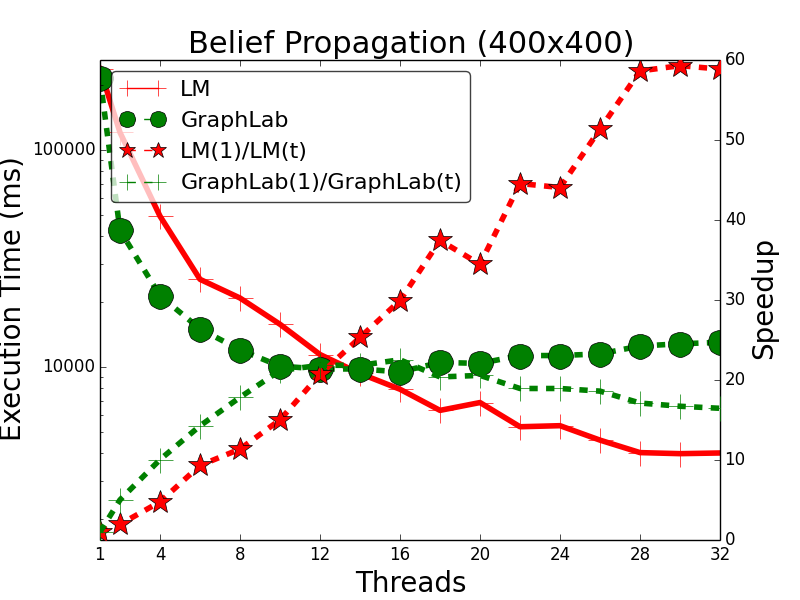
\includegraphics[width=\textwidth]{experiments/threads/cmp-fifo-belief-propagation-400.png}
           \mycap{Comparing the scalability of LM and of GraphLab's
              \textbf{fifo} scheduler}
           \label{fig:threads:splash_fifo}
        \end{subfigure}
        ~ ~
        \begin{subfigure}[b]{\plotsize\textwidth}
           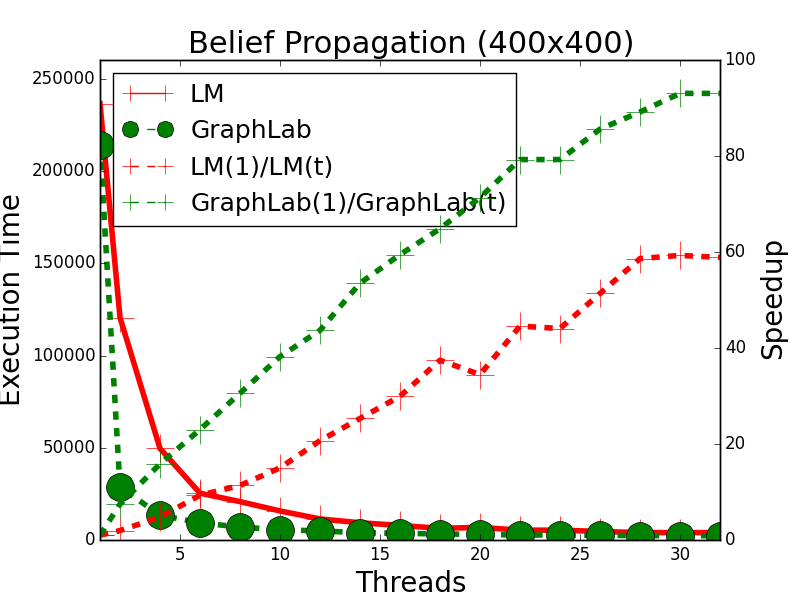
\includegraphics[width=\textwidth]{experiments/threads/cmp-multi-belief-propagation-400.png}
           \mycap{Comparing the scalability of LM and of GraphLab's
              \textbf{multiqueue} scheduler}
           \label{fig:threads:splash_multi}
        \end{subfigure} \\
        \mycap{Comparing the scalability of LM against GraphLab's (\textbf{fifo}
        and \textbf{multiqueue} schedulers.}
        \label{fig:threads:results_splash}
\end{figure}

The scalability and run time of the SBP program is compared in
Fig.~\ref{fig:threads:results_splash_ratio}(a). When compared to LM, GraphLab is
about twice as fast and that advantage is constant across the number of threads
since both systems have a similar scalability. Finally, in
Fig.~\ref{fig:threads:results_splash_ratio}(b), we compare the performance of
LBP program against the performance of SBP by calculating $LBP(t)/SBP(t)$, where
$LBP(t)$ is the run time of LBP for $t$ threads, while $SBP(t)$ is the run time
of SBP for $t$ threads. For LM, SBP improves noticeably over LBP but that
advantage is reduced as the number of threads increases. The same behavior is
also seen in GraphLab's \textbf{multiqueue} scheduler but since this scheduler
works so well under a shared memory setting, the advantages of the
\textbf{splash} scheduler are reduced. LM is able to improve its performance
with SBP since it is a slower language and reducing the number of facts derived
provides an improved performance.

\begin{figure}[]
        \centering
        \begin{subfigure}[b]{\plotsize\textwidth}
        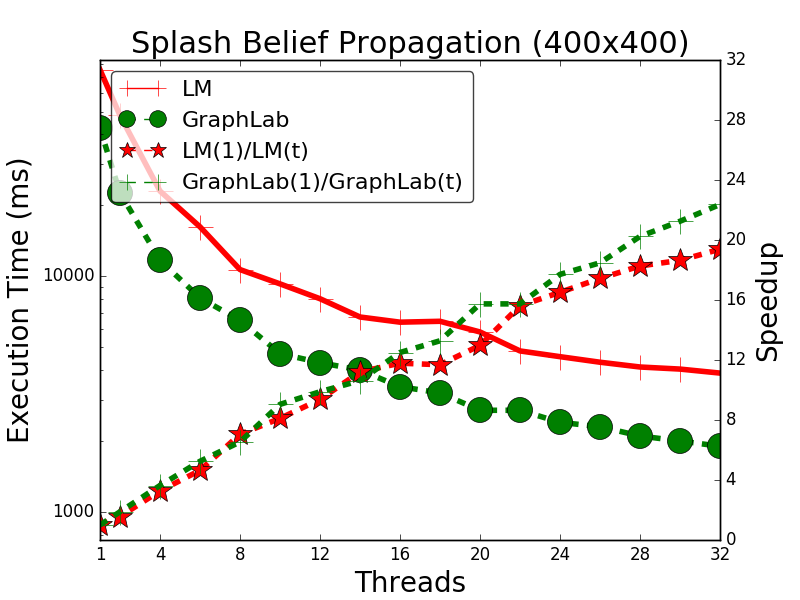
\includegraphics[width=\textwidth]{experiments/threads/cmp-splash-bp-400.png}
        \mycap{Measuring and comparing the performance of SBP in LM and
           the same program using GraphLab's \textbf{splash} scheduler.}
           \label{fig:threads:results_splash_final}
        \end{subfigure}~ ~
        \begin{subfigure}[b]{\plotsize\textwidth}
           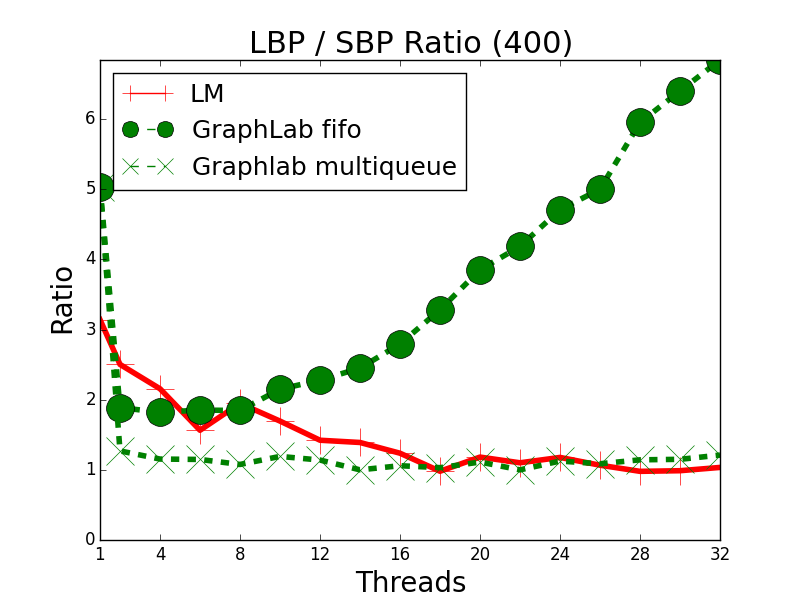
\includegraphics[width=\textwidth]{experiments/threads/cmp-ratio-belief-propagation-400.png}
           \mycap{Comparing the GraphLab's \textbf{splash}
           scheduler against the \textbf{fifo} and the \textbf{multiqueue}
        schedulers.}
           \label{fig:threads:splash_ratio_fifo}
        \end{subfigure}\\
        \mycap{Evaluating the performance of SBP over LBP in LM and GraphLab.}
        \label{fig:threads:results_splash_ratio}
\end{figure}
